\documentclass[border=1pt]{standalone}
\usepackage{newtxtext,newtxmath}
\usepackage{pgfplots}
\pgfplotsset{compat=1.18}
\definecolor{obs}{HTML}{D55E00}
\definecolor{sens}{HTML}{0072B2}
\begin{document}
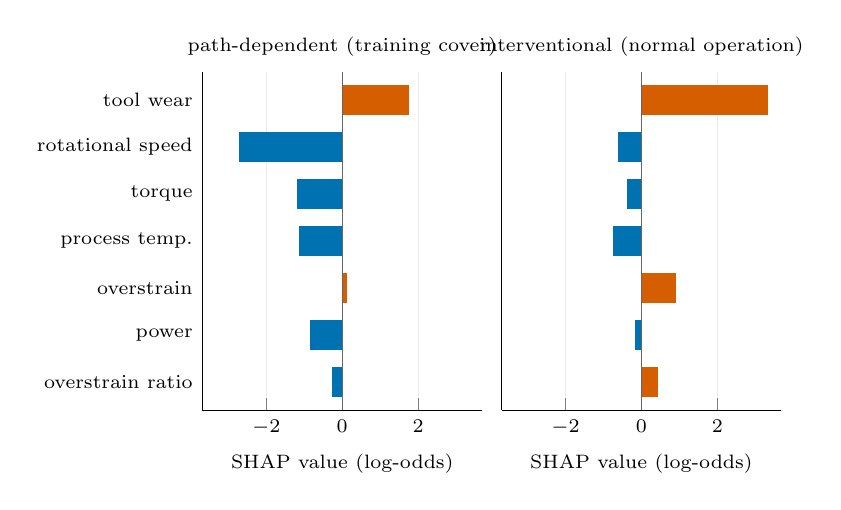
\begin{tikzpicture}
\begin{axis}[name=P, yticklabels={{tool wear},{rotational speed},{torque},{process temp.},{overstrain},{power},{overstrain ratio}}, width=3.55cm, height=4.3cm, scale only axis,
  xmin=-3.678, xmax=3.678, ymin=-0.6, ymax=6.6, y dir=reverse,
  ytick={0,...,6}, tick label style={font=\scriptsize}, ytick style={draw=none},
  title={path-dependent (training cover)}, title style={font=\scriptsize, yshift=-4pt}, xlabel={SHAP value (log-odds)},
  xlabel style={font=\scriptsize}, xmajorgrids, grid style={black!8}, axis y line*=left, axis x line*=bottom]
\addplot[draw=none] coordinates {(0,0)};
\fill[obs] (axis cs:0,-0.32) rectangle (axis cs:1.7677,0.32);
\fill[sens] (axis cs:0,0.6799999999999999) rectangle (axis cs:-2.7114,1.32);
\fill[sens] (axis cs:0,1.68) rectangle (axis cs:-1.2018,2.32);
\fill[sens] (axis cs:0,2.68) rectangle (axis cs:-1.1294,3.32);
\fill[obs] (axis cs:0,3.68) rectangle (axis cs:0.1277,4.32);
\fill[sens] (axis cs:0,4.68) rectangle (axis cs:-0.8566,5.32);
\fill[sens] (axis cs:0,5.68) rectangle (axis cs:-0.2750,6.32);
\draw[black!60, line width=0.5pt] (axis cs:0,-0.6) -- (axis cs:0,6.6);
\end{axis}
\begin{axis}[name=I, at={(P.east)}, anchor=west, xshift=0.25cm, yticklabels={}, width=3.55cm, height=4.3cm, scale only axis,
  xmin=-3.678, xmax=3.678, ymin=-0.6, ymax=6.6, y dir=reverse,
  ytick={0,...,6}, tick label style={font=\scriptsize}, ytick style={draw=none},
  title={interventional (normal operation)}, title style={font=\scriptsize, yshift=-4pt}, xlabel={SHAP value (log-odds)},
  xlabel style={font=\scriptsize}, xmajorgrids, grid style={black!8}, axis y line*=left, axis x line*=bottom]
\addplot[draw=none] coordinates {(0,0)};
\fill[obs] (axis cs:0,-0.32) rectangle (axis cs:3.3434,0.32);
\fill[sens] (axis cs:0,0.6799999999999999) rectangle (axis cs:-0.6043,1.32);
\fill[sens] (axis cs:0,1.68) rectangle (axis cs:-0.3732,2.32);
\fill[sens] (axis cs:0,2.68) rectangle (axis cs:-0.7488,3.32);
\fill[obs] (axis cs:0,3.68) rectangle (axis cs:0.9014,4.32);
\fill[sens] (axis cs:0,4.68) rectangle (axis cs:-0.1636,5.32);
\fill[obs] (axis cs:0,5.68) rectangle (axis cs:0.4445,6.32);
\draw[black!60, line width=0.5pt] (axis cs:0,-0.6) -- (axis cs:0,6.6);
\end{axis}
\end{tikzpicture}
\end{document}
